%
% tikztemplate.tex
%
% (c) 2018 Prof Dr Andreas Müller, Hochschule Rapperswil
%
\documentclass[tikz,12pt]{standalone}
\usepackage{times}
\usepackage{amsmath}
\usepackage{txfonts}
\usepackage[utf8]{inputenc}
\usepackage{graphics}
\usepackage{color}
\usepackage{pifont}
\usetikzlibrary{arrows,intersections,math,calc}
\begin{document}

\def\punkt#1{
        \fill[color=white] #1 circle[radius=0.08];
        \draw #1 circle[radius=0.08];
}

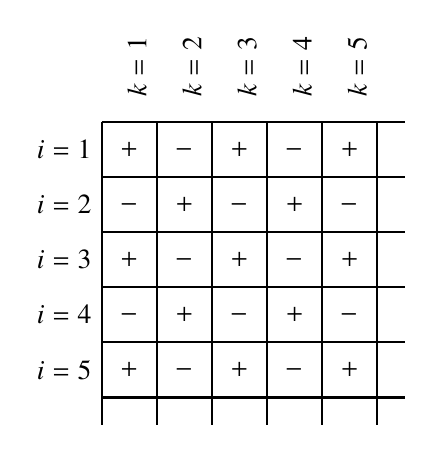
\begin{tikzpicture}[>=latex, thick, scale=0.7]
\draw (-0.5,0.5)--(5,0.5);
\node at (0,0) {$+$};
        \node at (1,0) {$-$};
                \node at (2,0) {$+$};
                        \node at (3,0) {$-$};
                                \node at (4,0) {$+$};
\draw (-0.5,-0.5)--(5,-0.5);
\node at (0,-1) {$-$};
        \node at (1,-1) {$+$};
                \node at (2,-1) {$-$};
                        \node at (3,-1) {$+$};
                                \node at (4,-1) {$-$};
\draw (-0.5,-1.5)--(5,-1.5);
\node at (0,-2) {$+$};
        \node at (1,-2) {$-$};
                \node at (2,-2) {$+$};
                        \node at (3,-2) {$-$};
                                \node at (4,-2) {$+$};
\draw (-0.5,-2.5)--(5,-2.5);
\node at (0,-3) {$-$};
        \node at (1,-3) {$+$};
                \node at (2,-3) {$-$};
                        \node at (3,-3) {$+$};
                                \node at (4,-3) {$-$};
\draw (-0.5,-3.5)--(5,-3.5);
\node at (0,-4) {$+$};
        \node at (1,-4) {$-$};
                \node at (2,-4) {$+$};
                        \node at (3,-4) {$-$};
                                \node at (4,-4) {$+$};
\draw (-0.5,-4.5)--(5,-4.5);

\draw (-0.5,0.5)--(-0.5,-5);
\draw ( 0.5,0.5)--( 0.5,-5);
\draw ( 1.5,0.5)--( 1.5,-5);
\draw ( 2.5,0.5)--( 2.5,-5);
\draw ( 3.5,0.5)--( 3.5,-5);
\draw ( 4.5,0.5)--( 4.5,-5);

\node at (-0.5, 0) [left] {$i=1$};
\node at (-0.5,-1) [left] {$i=2$};
\node at (-0.5,-2) [left] {$i=3$};
\node at (-0.5,-3) [left] {$i=4$};
\node at (-0.5,-4) [left] {$i=5$};

\node at (0.5,1.5) [rotate=90,above] {$k=1$};
\node at (1.5,1.5) [rotate=90,above] {$k=2$};
\node at (2.5,1.5) [rotate=90,above] {$k=3$};
\node at (3.5,1.5) [rotate=90,above] {$k=4$};
\node at (4.5,1.5) [rotate=90,above] {$k=5$};

\end{tikzpicture}

\end{document}
